\documentclass[journal, a4paper]{IEEEtran}

% some very useful LaTeX packages include:

%\usepackage{cite}      % Written by Donald Arseneau
                        % V1.6 and later of IEEEtran pre-defines the format
                        % of the cite.sty package \cite{} output to follow
                        % that of IEEE. Loading the cite package will
                        % result in citation numbers being automatically
                        % sorted and properly "ranged". i.e.,
                        % [1], [9], [2], [7], [5], [6]
                        % (without using cite.sty)
                        % will become:
                        % [1], [2], [5]--[7], [9] (using cite.sty)
                        % cite.sty's \cite will automatically add leading
                        % space, if needed. Use cite.sty's noadjust option
                        % (cite.sty V3.8 and later) if you want to turn this
                        % off. cite.sty is already installed on most LaTeX
                        % systems. The latest version can be obtained at:
                        % http://www.ctan.org/tex-archive/macros/latex/contrib/supported/cite/

\usepackage{graphicx}   % Written by David Carlisle and Sebastian Rahtz
                        % Required if you want graphics, photos, etc.
                        % graphicx.sty is already installed on most LaTeX
                        % systems. The latest version and documentation can
                        % be obtained at:
                        % http://www.ctan.org/tex-archive/macros/latex/required/graphics/
                        % Another good source of documentation is "Using
                        % Imported Graphics in LaTeX2e" by Keith Reckdahl
                        % which can be found as esplatex.ps and epslatex.pdf
                        % at: http://www.ctan.org/tex-archive/info/

%\usepackage{psfrag}    % Written by Craig Barratt, Michael C. Grant,
                        % and David Carlisle
                        % This package allows you to substitute LaTeX
                        % commands for text in imported EPS graphic files.
                        % In this way, LaTeX symbols can be placed into
                        % graphics that have been generated by other
                        % applications. You must use latex->dvips->ps2pdf
                        % workflow (not direct pdf output from pdflatex) if
                        % you wish to use this capability because it works
                        % via some PostScript tricks. Alternatively, the
                        % graphics could be processed as separate files via
                        % psfrag and dvips, then converted to PDF for
                        % inclusion in the main file which uses pdflatex.
                        % Docs are in "The PSfrag System" by Michael C. Grant
                        % and David Carlisle. There is also some information
                        % about using psfrag in "Using Imported Graphics in
                        % LaTeX2e" by Keith Reckdahl which documents the
                        % graphicx package (see above). The psfrag package
                        % and documentation can be obtained at:
                        % http://www.ctan.org/tex-archive/macros/latex/contrib/supported/psfrag/

%\usepackage{subfigure} % Written by Steven Douglas Cochran
                        % This package makes it easy to put subfigures
                        % in your figures. i.e., "figure 1a and 1b"
                        % Docs are in "Using Imported Graphics in LaTeX2e"
                        % by Keith Reckdahl which also documents the graphicx
                        % package (see above). subfigure.sty is already
                        % installed on most LaTeX systems. The latest version
                        % and documentation can be obtained at:
                        % http://www.ctan.org/tex-archive/macros/latex/contrib/supported/subfigure/

\usepackage{url}        % Written by Donald Arseneau
                        % Provides better support for handling and breaking
                        % URLs. url.sty is already installed on most LaTeX
                        % systems. The latest version can be obtained at:
                        % http://www.ctan.org/tex-archive/macros/latex/contrib/other/misc/
                        % Read the url.sty source comments for usage information.

%\usepackage{stfloats}  % Written by Sigitas Tolusis
                        % Gives LaTeX2e the ability to do double column
                        % floats at the bottom of the page as well as the top.
                        % (e.g., "\begin{figure*}[!b]" is not normally
                        % possible in LaTeX2e). This is an invasive package
                        % which rewrites many portions of the LaTeX2e output
                        % routines. It may not work with other packages that
                        % modify the LaTeX2e output routine and/or with other
                        % versions of LaTeX. The latest version and
                        % documentation can be obtained at:
                        % http://www.ctan.org/tex-archive/macros/latex/contrib/supported/sttools/
                        % Documentation is contained in the stfloats.sty
                        % comments as well as in the presfull.pdf file.
                        % Do not use the stfloats baselinefloat ability as
                        % IEEE does not allow \baselineskip to stretch.
                        % Authors submitting work to the IEEE should note
                        % that IEEE rarely uses double column equations and
                        % that authors should try to avoid such use.
                        % Do not be tempted to use the cuted.sty or
                        % midfloat.sty package (by the same author) as IEEE
                        % does not format its papers in such ways.

\usepackage{amsmath}    % From the American Mathematical Society
                        % A popular package that provides many helpful commands
                        % for dealing with mathematics. Note that the AMSmath
                        % package sets \interdisplaylinepenalty to 10000 thus
                        % preventing page breaks from occurring within multiline
                        % equations. Use:
%\interdisplaylinepenalty=2500
                        % after loading amsmath to restore such page breaks
                        % as IEEEtran.cls normally does. amsmath.sty is already
                        % installed on most LaTeX systems. The latest version
                        % and documentation can be obtained at:
                        % http://www.ctan.org/tex-archive/macros/latex/required/amslatex/math/
\usepackage{listings}

\usepackage{xcolor}

\usepackage{float}


% Other popular packages for formatting tables and equations include:

%\usepackage{array}
% Frank Mittelbach's and David Carlisle's array.sty which improves the
% LaTeX2e array and tabular environments to provide better appearances and
% additional user controls. array.sty is already installed on most systems.
% The latest version and documentation can be obtained at:
% http://www.ctan.org/tex-archive/macros/latex/required/tools/

% V1.6 of IEEEtran contains the IEEEeqnarray family of commands that can
% be used to generate multiline equations as well as matrices, tables, etc.

% Also of notable interest:
% Scott Pakin's eqparbox package for creating (automatically sized) equal
% width boxes. Available:
% http://www.ctan.org/tex-archive/macros/latex/contrib/supported/eqparbox/

% *** Do not adjust lengths that control margins, column widths, etc. ***
% *** Do not use packages that alter fonts (such as pslatex).         ***
% There should be no need to do such things with IEEEtran.cls V1.6 and later.


% Your document starts here!
\begin{document}
\begin{titlepage}

\newcommand{\HRule}{\rule{\linewidth}{0.5mm}} % Defines a new command for the horizontal lines, change thickness here

\center % Center everything on the page
 %----------------------------------------------------------------------------------------
%	LOGO SECTION
%----------------------------------------------------------------------------------------

~\\[1cm]

\includegraphics{SCUT.png}\\[2cm] % Include a department/university logo - this will require the graphicx package

%----------------------------------------------------------------------------------------
%	TITLE SECTION
%----------------------------------------------------------------------------------------

\HRule \\[1cm]
{ \huge \bfseries The Experiment Report of \textit{Machine Learning} }\\[0.6cm] % Title of your document
\HRule \\[2cm]
%----------------------------------------------------------------------------------------
%	HEADING SECTIONS
%----------------------------------------------------------------------------------------


\textsc{\LARGE \textbf{School:} School of Software Engineering}\\[1cm]
\textsc{\LARGE \textbf{Subject:} Software Engineering}\\[2cm] 

 
%----------------------------------------------------------------------------------------
%	AUTHOR SECTION
%----------------------------------------------------------------------------------------

\begin{minipage}{0.4\textwidth}
\begin{flushleft} \large
\emph{Author:}\\
 Chen Han % Your name
\end{flushleft}
\end{minipage}
~
\begin{minipage}{0.4\textwidth}
\begin{flushright} \large
\emph{Supervisor:} \\
Mingkui Tan% Supervisor's Name
\end{flushright}
\end{minipage}\\[2cm]
~
\begin{minipage}{0.4\textwidth}
\begin{flushleft} \large
\emph{Student ID:}\\
201936380086
\end{flushleft}
\end{minipage}
~
\begin{minipage}{0.4\textwidth}
\begin{flushright} \large
\emph{Grade:} \\
Class 1, Grade 2019
\end{flushright}
\end{minipage}\\[2cm]

% If you don't want a supervisor, uncomment the two lines below and remove the section above
%\Large \emph{Author:}\\
%John \textsc{Smith}\\[3cm] % Your name

%----------------------------------------------------------------------------------------
%	DATE SECTION
%----------------------------------------------------------------------------------------

{\large \today}\\[2cm] % Date, change the \today to a set date if you want to be precise

 
%----------------------------------------------------------------------------------------

\vfill % Fill the rest of the page with whitespace

\end{titlepage}

% Define document title and author
	\title{Logistic Regression and Support Vector Machine}
	\maketitle

% Write abstract here
\begin{abstract}
Further understand the principles of Logistic Regression and Support Vector Machine and practice on larger data.
\end{abstract}

% Each section begins with a \section{title} command
\section{Introduction}
	% \PARstart{}{} creates a tall first letter for this first paragraph
\PARstart{I}{n} order to further understand the conception of Logistic Regression and Support Vector Machine, we compare differences and relationships between Logistic regression and linear classification. We use dataset a9a of LIBSVM Data. Using SGD and Adam to optimize the efficiency.

% Main Part
\section{Methods and Theory}
\subsection{Logistic Regression and Batch Stochastic Gradient Descent}
We use probability function below:
\begin{equation}
	\begin{aligned}
	\nonumber
		h_w(x)&=g(z)\\
		&=g(\sum_{i=1}^mw_ix_i)\\
		&=g(w^Tx)
	\end{aligned}
\end{equation}
Here, $z=w^Tx$, $g(\cdot)$ is a logistic function:
$$g(z)=\frac{1}{1+e^{-z}} $$
The function is a continuous function. If $z\to+\infty$, then $g(z)\to1$ and if $z\to-\infty$, then $g(z)\to0$.\\
We define the threshold at 0.5, if $g(W^T X_i) \textgreater 0.5$ , we thought it's positive, or it's negative.\par
We would like to get:
\begin{equation}
	\begin{aligned}
	\nonumber
		\max\prod_{i=1}^n & \iff \max \log(\prod_{i=1}^nP(y_i|x_i))\\
		& \iff \min-\frac{1}{n}\sum_{i=1}^n\log P(y_i|x_i)\\
		& \iff  \min\frac{1}{n}\sum_{i=1}^n\frac{1}{\log P(y_i|x_i)}\\
		& \quad \equiv \quad min \frac{1}{n}\sum_{i=1}^n\log\frac{1}{g(y_iw^Tx_i)}\\
		& \quad \equiv \quad min \frac{1}{n}\sum_{i=1}^n\log(1+e^{-y_iw^Tx_i})\\
		& \quad \equiv \quad \min\mathcal{L}(W)
	\end{aligned}
\end{equation}
So we have loss function below:

$$ \min \mathcal{L} oss(W) = \frac{1}{n} \sum_{i=1}^n log(1+e^{-y_i W^T X_i})$$
In order to avoid overfitting, we rewrite this equation by regular item $\frac{\lambda}{2} \parallel W \parallel^2$, then we have:
$$ \min \mathcal{J}(W) = \frac{1}{n} \sum_{i=1}^n log(1+e^{-y_i W^T X_i}) + \frac{\lambda}{2} \parallel W \parallel^2$$ \par

We calculate gradient with formula below:
$$  \frac{\partial \mathcal{J}(W)}{\partial W} = -\frac{1}{n} \sum_{i=1}^n \frac{y_i X_i e^{-y_i W^T X_i}}{1+e^{-y_i W^T X_i}} + \lambda W$$


\subsection{Support Vector Machine}
We want to optimize the problem:
\begin{equation}
	\begin{aligned}
	\nonumber
		\min_{w,b,\xi_i}\frac{\parallel w \parallel^2}{2}+\frac{C}{n}\sum_{i=1}{n}\xi_i
	\end{aligned}
\end{equation}
$$s.t.\quad\quad y_i(w^Tx_i+b)\geq 1-\xi_i, \quad\forall \xi_i\geq0, i=1,2,\cdots ,n$$
where C is a hyperparameter:\\

\centerline{-small C makes constraints easy to be ignored}\centerline{-large C makes constraints hard to be ignored}	


\begin{equation}
	\begin{aligned}
	\nonumber
		if\quad 1-y_i(w^Tx_i+b)\geq 0, \quad \xi_i &=1-y_i(w^Tx_i+b)\\
		if\quad 1-y_i(w^Tx_i+b)\leq 0, \quad \xi_i &=0\\
	\end{aligned}
\end{equation}
So, we rewrite $\xi_i$ as:\\
$$\xi_i=\max(0,1-y_i(w^Tx_i+b))$$
The optimization problem becomes:
\begin{equation}
	\begin{aligned}
	\nonumber
		\min_{w,b,\xi_i}\frac{\parallel w \parallel^2}{2}+\frac{C}{n}\sum_{i=1}{n}\max{(0,1-y_i(w^Tx_i+b))}
	\end{aligned}
\end{equation}
Then we have the loss function:
$$ \min_{W, b} \mathcal{L}(W, b)= \frac{\parallel W \parallel^2}{2} + \frac{C}{n} \sum_{i=1}^n max(0, 1-y_i(W^T X_i + b))$$
To minimize a loss function $L(w, b)$, use the iterative update:
\begin{equation}
	\begin{aligned}
		w&=w-\eta\bigtriangledown_w L(w, b)\\
		b&=b-\eta\bigtriangledown_b L(w, b)\\
	\end{aligned}
\end{equation}
where $\eta$ is the learning rate.\\
We define threshold value at 0, if $\mathcal{f}(W^T X_i+b) \textgreater 0$, it's positive, or it's negative.\\
Then we have gradient descent with batch algorithm that uses all examples:
$$ \frac{\partial \mathcal{L}(W, b)}{\partial W} = \begin{cases}
-y_i X_i, & 1-y_i(W^T X_i + b) \ge 0 \\
0, &1-y_i(W^T X_i + b) < 0
\end{cases}$$
$$ \frac{\partial \mathcal{L}(W, b)}{\partial b} = \begin{cases}
-y_i, & 1-y_i(W^T X_i + b) \ge 0 \\
0, &1-y_i(W^T X_i + b) < 0
\end{cases}$$


\section{Experiments}
\subsection{Dataset}
Experiment uses a9a of LIBSVM Data, including 32561/16281(testing) samples and each sample has 123/123 (testing) features.

\subsection{Implementation}

	% You can reference tables and figure by using the \ref{label} command. Each table and figure needs to have a UNIQUE label.
	

	% This is how you define a table: the [!hbt] means that LaTeX is forced (by the !) to place the table exactly here (by h), or if that doesnt work because of a pagebreak or so, it tries to place the table to the bottom of the page (by b) or the top (by t).

1. Load the experiment data. Using load\_svmlight\_file function in sklearn library, adding one column by yourself or specify the n\_features to be 123 when using the function to avoid values of last column all zero to be ignored.\par
2. write Loss-calculating function for Logistic Regression.\par
\lstset{language=python}
\lstset{
	breaklines,
    numbers=left, 
    numberstyle= \tiny, 
    keywordstyle= \color{ blue!70},
    commentstyle= \color{red!50!green!50!blue!50}, 
    frame=shadowbox,
    rulesepcolor= \color{ red!20!green!20!blue!20} ,
    escapeinside=``, 
    xleftmargin=2em, aboveskip=1em,
    framexleftmargin=2em
}
3. Write sigmoid function.\par

4. Write validation calculating function for Logistic Regression.\par

5. Calculating gradient with formula above for Logistic Regression.

6. Write Logistic Regression function.\par
\begin{lstlisting}
def Logistic_Regression(X, Y, learning_rate, lamda, epoch, batch):
    loss = []
    acc = []
    W = np.random.rand(X.shape[1], 1)
    for i in tqdm(range(epoch), desc="Training pass: ", leave=True):
        bat = np.random.choice(X.shape[0], batch)
        X_batch = X[bat]
        Y_batch = Y[bat]
        gradient = calc_gradient_A(X_batch, Y_batch, W, lamda)
        W = W - learning_rate*gradient
        loss.append(calc_loss_A(X, Y, W))
        acc.append(calc_validation_A(W))
    return W, loss, acc
\end{lstlisting}\par
7. Write Logistic Regression function with Adam optimization.\par
\begin{lstlisting}
def Logistic_Regression_Adam(X, Y, learning_rate, lamda, epoch, batch, eps=1e-8, beta1=0.9, beta2=0.999):
    loss = []
    acc = []
    m = 0
    v = 0
    W = np.random.rand(X.shape[1], 1)
    for i in tqdm(range(epoch), desc="Training pass: ", leave=True):
        bat = np.random.choice(X.shape[0], batch)
        X_batch = X[bat]
        Y_batch = Y[bat]
        gradient = calc_gradient_A(X_batch, Y_batch, W, lamda)
        m = beta1 * m + (1 - beta1) * gradient
        v = beta2 * v + (1 - beta2) * (gradient ** 2)
        W = W - learning_rate * m / (np.sqrt(v) + eps)
        loss.append(calc_loss_A(X, Y, W))
        acc.append(calc_validation_A(W))
    return W, loss, acc
\end{lstlisting}\par
8. Define the function to calculate loss for SVM.\par

9. Write validation calculating function for SVM.\par

10. Calculating gradient with formula above for SVM.\par

11. Define the SVM classifier with Stochastic Gradient Descent.
\begin{lstlisting}
def SVM_classifier(X, Y, c, epoch, batch, learning_rate):
    loss = []
    acc = []
    W = np.random.rand(X.shape[1], 1)
    b = 0
    for i in tqdm(range(epoch), desc="Training pass: ", leave=True):
        bat = np.random.choice(X.shape[0], batch)
        X_batch = X[bat]
        Y_batch = Y[bat]
        gradient_W, gradient_b = calc_gradient_B(X_batch, Y_batch, W, b, c)
        W = W - learning_rate * gradient_W
        b = b - learning_rate * gradient_b
        loss.append(calc_loss_B(X, Y, W, b, c))
        acc.append(calc_validation_B(W, b))
    return W, loss, acc
\end{lstlisting}
12. Rewrite SVM classifier with Adam.\par
\begin{lstlisting}
def SVM_classifier_Adam(X, Y, c, epoch, batch, learning_rate, eps=1e-8, beta1=0.9, beta2=0.999):
    loss = []
    acc = []
    W = np.random.rand(X.shape[1], 1)
    b = 0
    mW = 0
    vW = 0
    mb = 0
    vb = 0
    for i in tqdm(range(epoch), desc="Training pass: ", leave=True):
        bat = np.random.choice(X.shape[0], batch)
        X_batch = X[bat]
        Y_batch = Y[bat]
        gradient_W, gradient_b = calc_gradient_B(X_batch, Y_batch, W, b, c)
        mW = beta1 * mW + (1 - beta1) * gradient_W
        vW = beta2 * vW + (1 - beta2) * (gradient_W ** 2)
        W = W - learning_rate * mW / (np.sqrt(vW) + eps)
        mb = beta1 * mb + (1 - beta1) * gradient_b
        vb = beta2 * vb + (1 - beta2) * (gradient_b ** 2)
        b = b - learning_rate * mb / (np.sqrt(vb) + eps)
        loss.append(calc_loss_B(X, Y, W, b, c))
        acc.append(calc_validation_B(W, b))
    return W, loss, acc
\end{lstlisting}
13. Get all the solutions.\par

	% If you have questions about how to write mathematical formulas in LaTeX, please read a LaTeX book or the 'Not So Short Introduction to LaTeX': tobi.oetiker.ch/lshort/lshort.pdf
	\begin{table}[!hbt]
		% Center the table
		\begin{center}
		% Title of the table
		\caption{Training speed}
		\label{tab:simParameters}
		% Table itself: here we have two columns which are centered and have lines to the left, right and in the middle: |c|c|
		\begin{tabular}{|c|c|}
			% To create a horizontal line, type \hline
			% To end a column type &
			% For a linebreak type \\
			\hline
			function & speed \\
			\hline
			Logistic\_Regression & 11.54it/s\\
			\hline
			Logistic\_Regression\_Adam & 11.42it/s\\
			\hline
			SVM\_classifier & 6.44it/s\\
			\hline
			SVM\_classifier\_Adam & 6.22it/s\\
			\hline
		\end{tabular}
		\end{center}
	\end{table}


	% This is how you include a eps figure in your document. LaTeX only accepts EPS or TIFF files.
	\begin{figure}[!hbt]
		% Center the figure.
		\begin{center}
		% Include the eps file, scale it such that it's width equals the column width. You can also put width=8cm for example...
		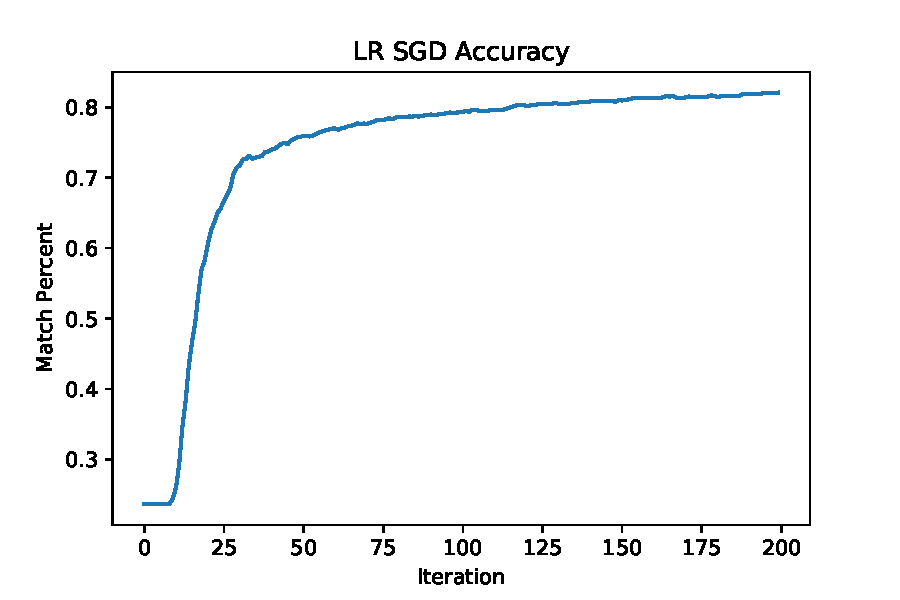
\includegraphics[width=\columnwidth]{lab2_lr_sgd_acc}
		% Create a subtitle for the figure.
		\caption{Accuracy of Logistic\_Regression with SGD.}
		% Define the label of the figure. It's good to use 'fig:title', so you know that the label belongs to a figure.
		\end{center}
	\end{figure}
		% This is how you include a eps figure in your document. LaTeX only accepts EPS or TIFF files.
	\begin{figure}[!hbt]
		% Center the figure.
		\begin{center}
		% Include the eps file, scale it such that it's width equals the column width. You can also put width=8cm for example...
		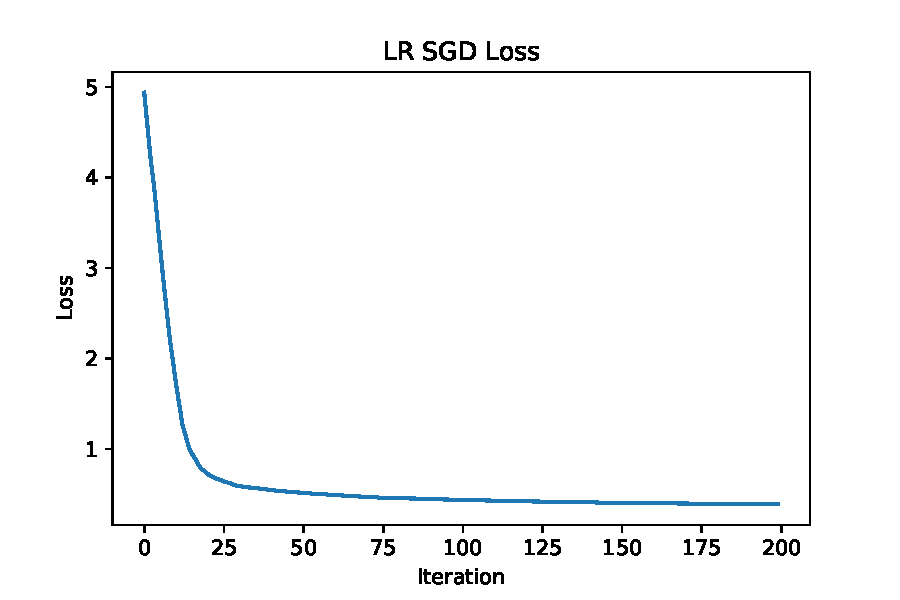
\includegraphics[width=\columnwidth]{lab2_lr_sgd_loss}
		% Create a subtitle for the figure.
		\caption{Loss of Logistic\_Regression with SGD.}
		% Define the label of the figure. It's good to use 'fig:title', so you know that the label belongs to a figure.
		\end{center}
	\end{figure}
	
	\begin{figure}[!hbt]
		% Center the figure.
		\begin{center}
		% Include the eps file, scale it such that it's width equals the column width. You can also put width=8cm for example...
		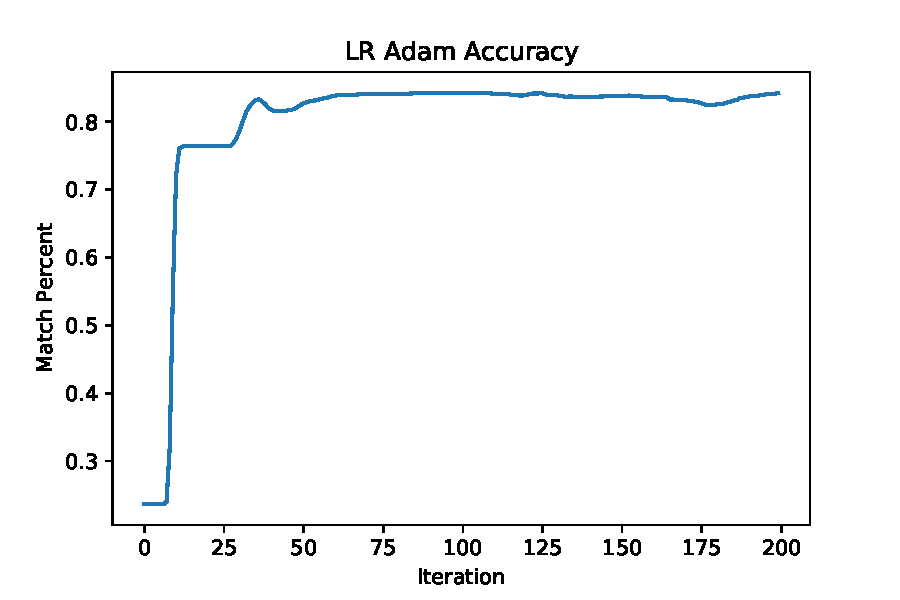
\includegraphics[width=\columnwidth]{lab2_lr_adam_acc}
		% Create a subtitle for the figure.
		\caption{Accuracy of Logistic\_Regression with adam.}
		% Define the label of the figure. It's good to use 'fig:title', so you know that the label belongs to a figure.
		\end{center}
	\end{figure}
		% This is how you include a eps figure in your document. LaTeX only accepts EPS or TIFF files.
	\begin{figure}[!hbt]
		% Center the figure.
		\begin{center}
		% Include the eps file, scale it such that it's width equals the column width. You can also put width=8cm for example...
		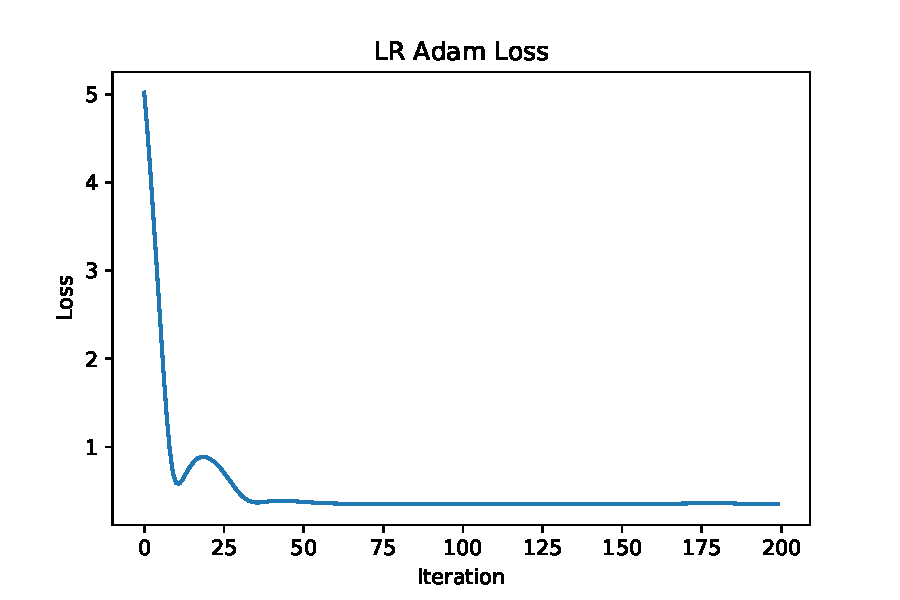
\includegraphics[width=\columnwidth]{lab2_lr_adam_loss}
		% Create a subtitle for the figure.
		\caption{Loss of Logistic\_Regression with adam.}
		% Define the label of the figure. It's good to use 'fig:title', so you know that the label belongs to a figure.
		\end{center}
	\end{figure}
	
	\begin{figure}[!hbt]
		% Center the figure.
		\begin{center}
		% Include the eps file, scale it such that it's width equals the column width. You can also put width=8cm for example...
		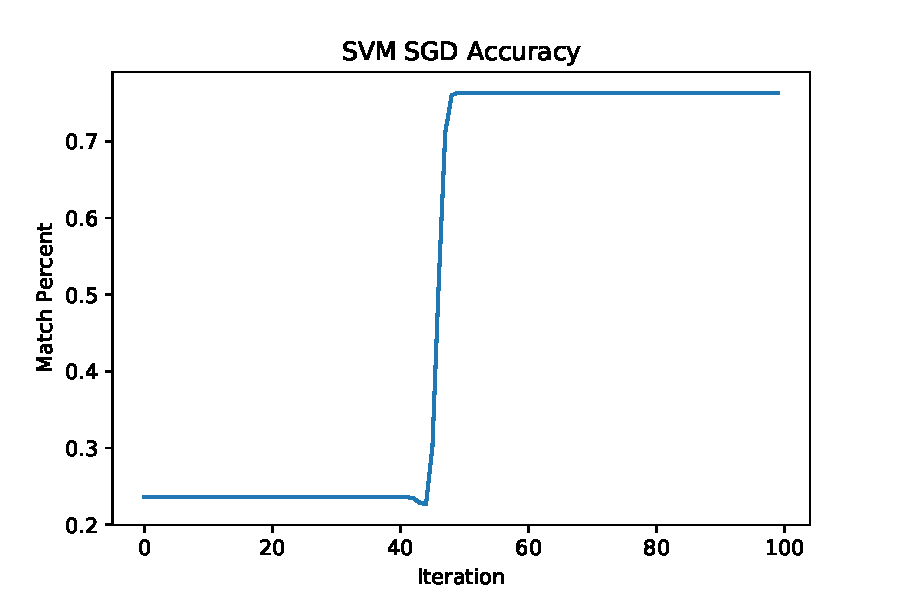
\includegraphics[width=\columnwidth]{lab2_svm_sgd_acc}
		% Create a subtitle for the figure.
		\caption{Accuracy of SVM with SGD.}
		% Define the label of the figure. It's good to use 'fig:title', so you know that the label belongs to a figure.
		\end{center}
	\end{figure}
		% This is how you include a eps figure in your document. LaTeX only accepts EPS or TIFF files.
	\begin{figure}[!hbt]
		% Center the figure.
		\begin{center}
		% Include the eps file, scale it such that it's width equals the column width. You can also put width=8cm for example...
		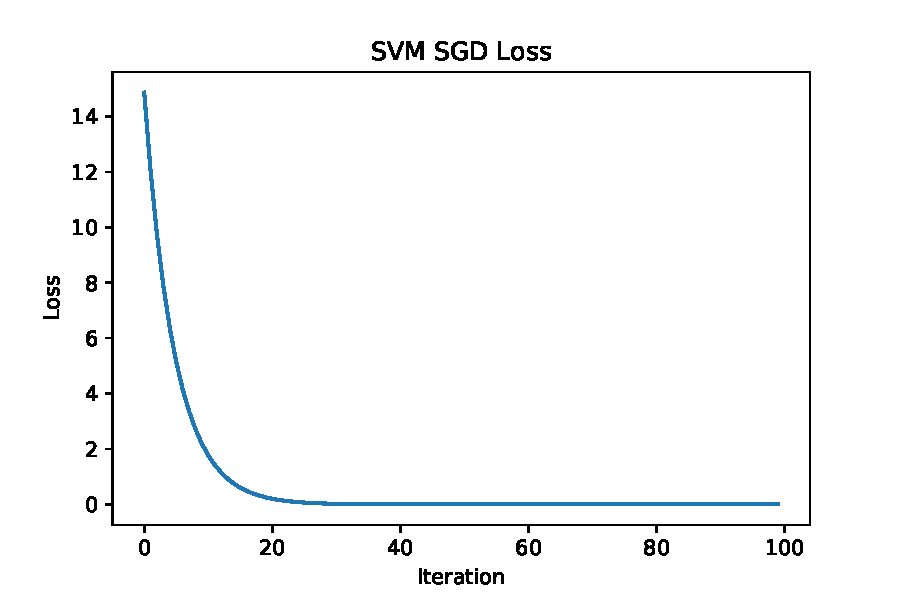
\includegraphics[width=\columnwidth]{lab2_svm_sgd_loss}
		% Create a subtitle for the figure.
		\caption{Loss of SVM with SGD.}
		% Define the label of the figure. It's good to use 'fig:title', so you know that the label belongs to a figure.
		\end{center}
	\end{figure}
	
	\begin{figure}[!hbt]
		% Center the figure.
		\begin{center}
		% Include the eps file, scale it such that it's width equals the column width. You can also put width=8cm for example...
		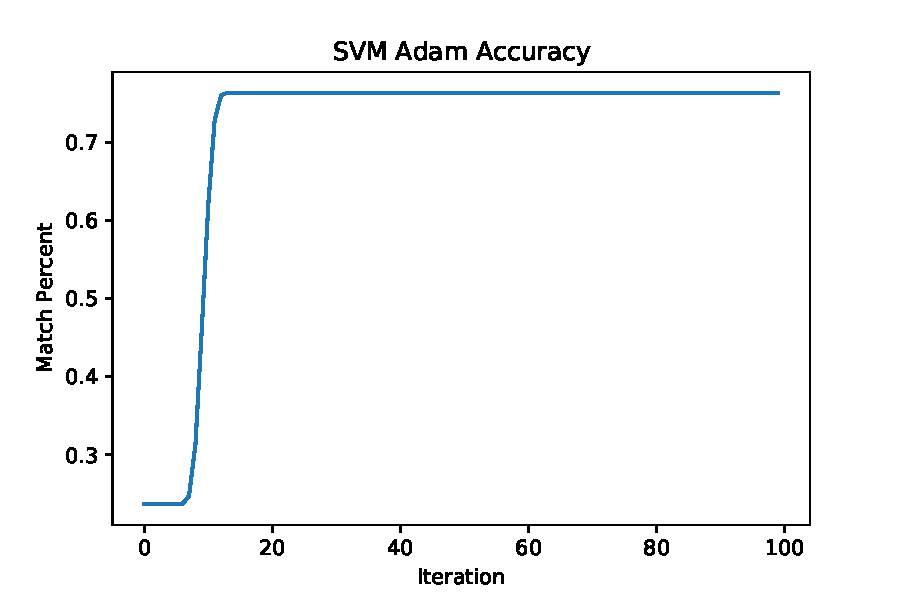
\includegraphics[width=\columnwidth]{lab2_svm_adam_acc}
		% Create a subtitle for the figure.
		\caption{Accuracy of SVM with adam.}
		% Define the label of the figure. It's good to use 'fig:title', so you know that the label belongs to a figure.
		\end{center}
	\end{figure}
		% This is how you include a eps figure in your document. LaTeX only accepts EPS or TIFF files.
	\begin{figure}[!hbt]
		% Center the figure.
		\centering
		% Include the eps file, scale it such that it's width equals the column width. You can also put width=8cm for example...
		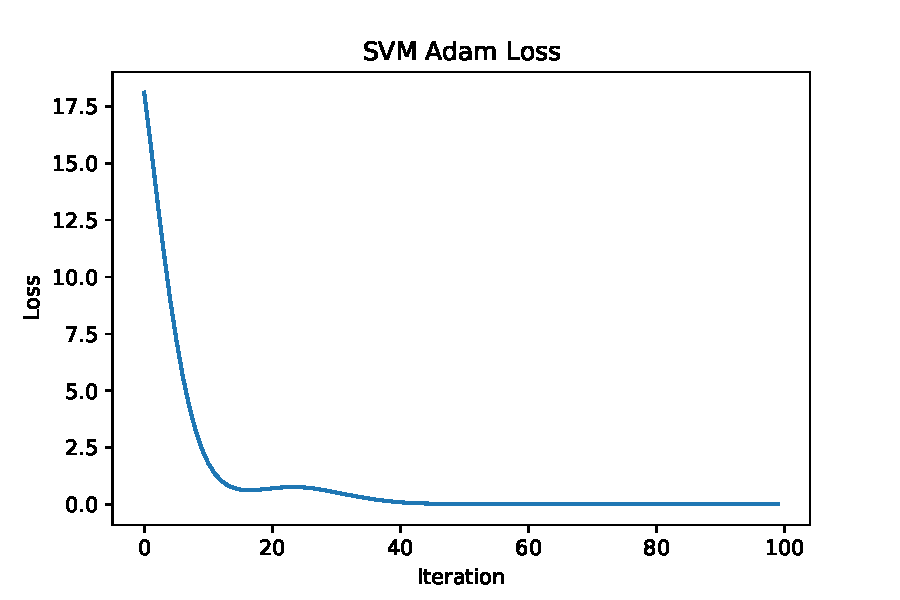
\includegraphics[width=\columnwidth]{lab2_svm_adam_loss}
		% Create a subtitle for the figure.
		\caption{Loss of SVM with adam.}
		% Define the label of the figure. It's good to use 'fig:title', so you know that the label belongs to a figure.
	\end{figure}


\section{Conclusion}
	In this experiment, I learnt the difference between  Logistic\_Regression and SVM while learnt the principle of them.



% Your document ends here!
\end{document}